\chapter{Code Overview}
Wannier90 can operate in two modes

\begin{enumerate}
\item Read in the overlaps and projections from file as computed 
inside a first-principles code. We expect this to be the most common route to using Wannier90.


\item As a set of library routines to be called from within a first-principles code. 
The first-principles code passes the overlaps and projections to the Wannier90 library routines
and in return gets the unitary transformation corresponding to Maximally Localised Wannier Functions.
This route should be used if the Wannier functions are needed within the first-principles code, for example
in post-LDA methods such as LDA+U or SIC. (this mode is under development)
\end{enumerate}


\begin{figure}
\begin{center}
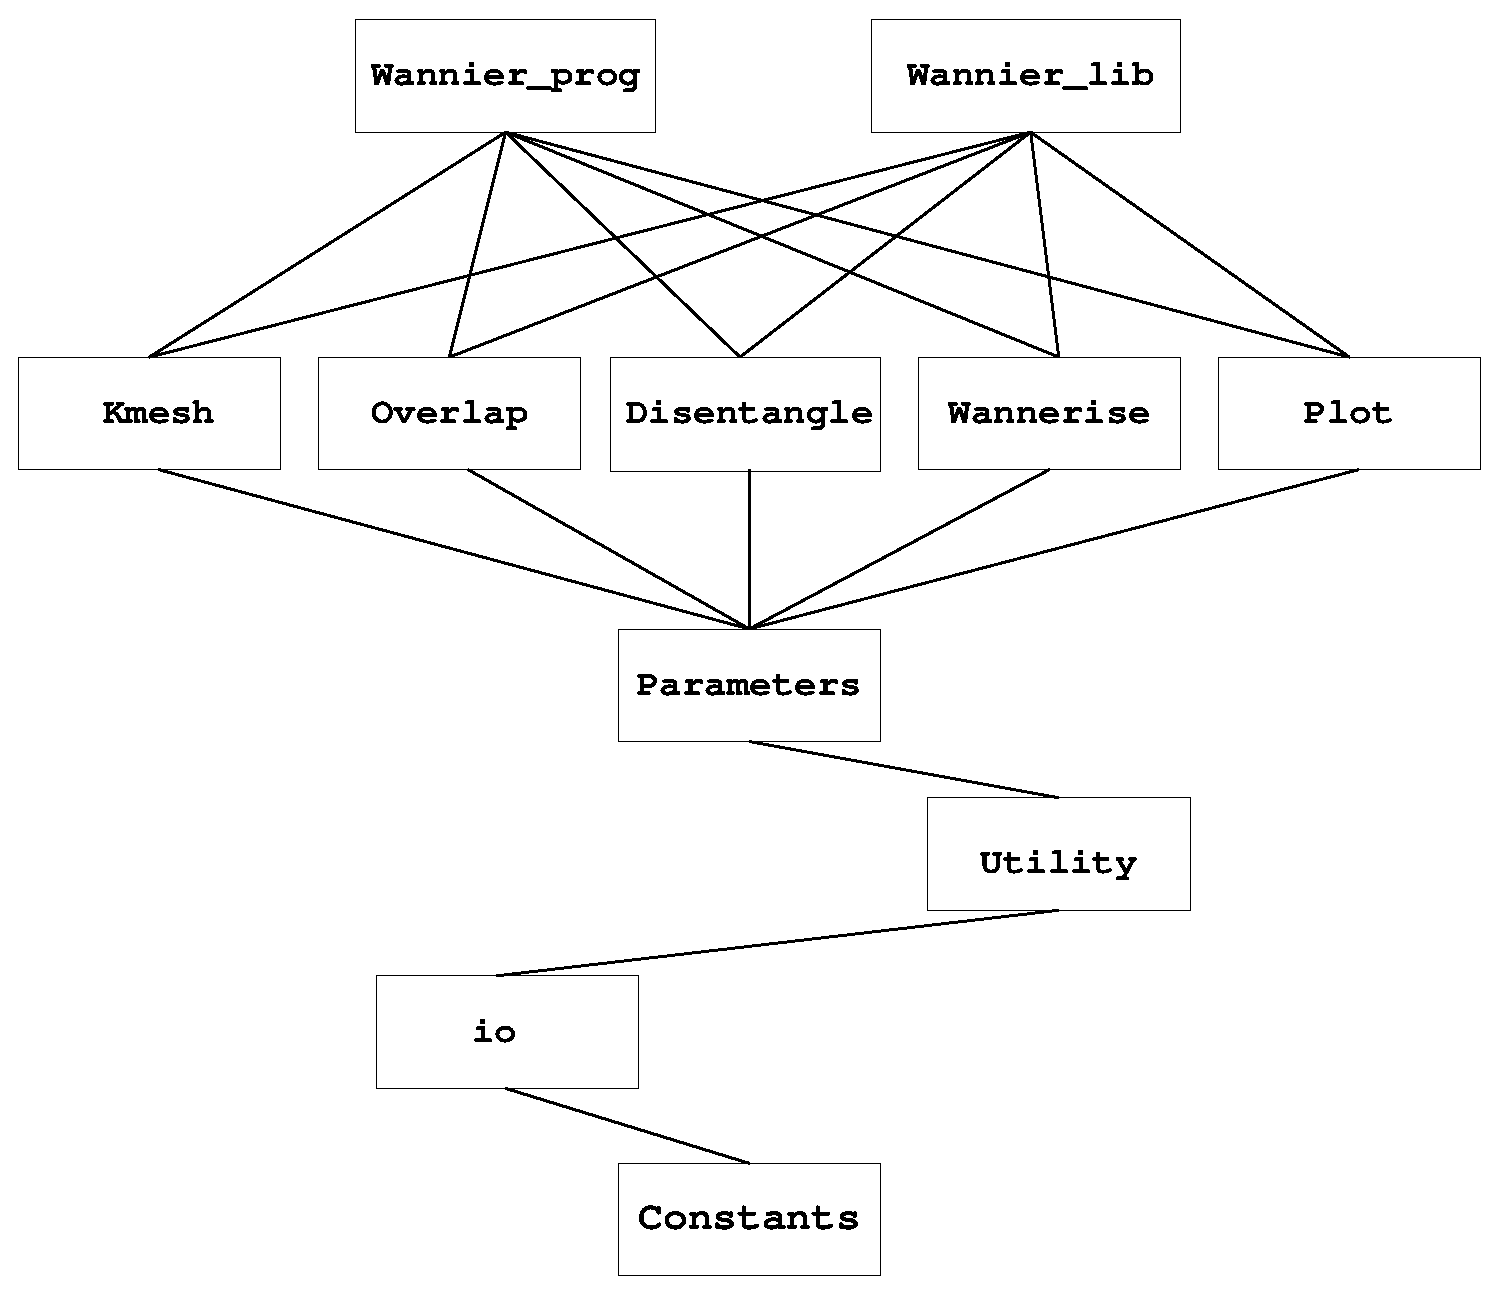
\includegraphics[width=5in]{overview.eps}
\caption{Schematic overview of the module structure of the Wannier90 code. Modules may only use data
and subroutines from lower modules.}
\label{structure}
\end{center}
\end{figure}
